% Options for packages loaded elsewhere
\PassOptionsToPackage{unicode}{hyperref}
\PassOptionsToPackage{hyphens}{url}
\PassOptionsToPackage{dvipsnames,svgnames,x11names}{xcolor}
\documentclass[
  11pt,
]{article}
\usepackage{xcolor}
\usepackage[margin=2.5cm]{geometry}
\usepackage{amsmath,amssymb}
\setcounter{secnumdepth}{-\maxdimen} % remove section numbering
\usepackage{iftex}
\ifPDFTeX
  \usepackage[T1]{fontenc}
  \usepackage[utf8]{inputenc}
  \usepackage{textcomp} % provide euro and other symbols
\else % if luatex or xetex
  \usepackage{unicode-math} % this also loads fontspec
  \defaultfontfeatures{Scale=MatchLowercase}
  \defaultfontfeatures[\rmfamily]{Ligatures=TeX,Scale=1}
\fi
\usepackage[]{charter}
\ifPDFTeX\else
  % xetex/luatex font selection
\fi
% Use upquote if available, for straight quotes in verbatim environments
\IfFileExists{upquote.sty}{\usepackage{upquote}}{}
\IfFileExists{microtype.sty}{% use microtype if available
  \usepackage[]{microtype}
  \UseMicrotypeSet[protrusion]{basicmath} % disable protrusion for tt fonts
}{}
\makeatletter
\@ifundefined{KOMAClassName}{% if non-KOMA class
  \IfFileExists{parskip.sty}{%
    \usepackage{parskip}
  }{% else
    \setlength{\parindent}{0pt}
    \setlength{\parskip}{6pt plus 2pt minus 1pt}}
}{% if KOMA class
  \KOMAoptions{parskip=half}}
\makeatother
\usepackage{color}
\usepackage{fancyvrb}
\newcommand{\VerbBar}{|}
\newcommand{\VERB}{\Verb[commandchars=\\\{\}]}
\DefineVerbatimEnvironment{Highlighting}{Verbatim}{commandchars=\\\{\}}
% Add ',fontsize=\small' for more characters per line
\usepackage{framed}
\definecolor{shadecolor}{RGB}{248,248,248}
\newenvironment{Shaded}{\begin{snugshade}}{\end{snugshade}}
\newcommand{\AlertTok}[1]{\textcolor[rgb]{0.94,0.16,0.16}{#1}}
\newcommand{\AnnotationTok}[1]{\textcolor[rgb]{0.56,0.35,0.01}{\textbf{\textit{#1}}}}
\newcommand{\AttributeTok}[1]{\textcolor[rgb]{0.13,0.29,0.53}{#1}}
\newcommand{\BaseNTok}[1]{\textcolor[rgb]{0.00,0.00,0.81}{#1}}
\newcommand{\BuiltInTok}[1]{#1}
\newcommand{\CharTok}[1]{\textcolor[rgb]{0.31,0.60,0.02}{#1}}
\newcommand{\CommentTok}[1]{\textcolor[rgb]{0.56,0.35,0.01}{\textit{#1}}}
\newcommand{\CommentVarTok}[1]{\textcolor[rgb]{0.56,0.35,0.01}{\textbf{\textit{#1}}}}
\newcommand{\ConstantTok}[1]{\textcolor[rgb]{0.56,0.35,0.01}{#1}}
\newcommand{\ControlFlowTok}[1]{\textcolor[rgb]{0.13,0.29,0.53}{\textbf{#1}}}
\newcommand{\DataTypeTok}[1]{\textcolor[rgb]{0.13,0.29,0.53}{#1}}
\newcommand{\DecValTok}[1]{\textcolor[rgb]{0.00,0.00,0.81}{#1}}
\newcommand{\DocumentationTok}[1]{\textcolor[rgb]{0.56,0.35,0.01}{\textbf{\textit{#1}}}}
\newcommand{\ErrorTok}[1]{\textcolor[rgb]{0.64,0.00,0.00}{\textbf{#1}}}
\newcommand{\ExtensionTok}[1]{#1}
\newcommand{\FloatTok}[1]{\textcolor[rgb]{0.00,0.00,0.81}{#1}}
\newcommand{\FunctionTok}[1]{\textcolor[rgb]{0.13,0.29,0.53}{\textbf{#1}}}
\newcommand{\ImportTok}[1]{#1}
\newcommand{\InformationTok}[1]{\textcolor[rgb]{0.56,0.35,0.01}{\textbf{\textit{#1}}}}
\newcommand{\KeywordTok}[1]{\textcolor[rgb]{0.13,0.29,0.53}{\textbf{#1}}}
\newcommand{\NormalTok}[1]{#1}
\newcommand{\OperatorTok}[1]{\textcolor[rgb]{0.81,0.36,0.00}{\textbf{#1}}}
\newcommand{\OtherTok}[1]{\textcolor[rgb]{0.56,0.35,0.01}{#1}}
\newcommand{\PreprocessorTok}[1]{\textcolor[rgb]{0.56,0.35,0.01}{\textit{#1}}}
\newcommand{\RegionMarkerTok}[1]{#1}
\newcommand{\SpecialCharTok}[1]{\textcolor[rgb]{0.81,0.36,0.00}{\textbf{#1}}}
\newcommand{\SpecialStringTok}[1]{\textcolor[rgb]{0.31,0.60,0.02}{#1}}
\newcommand{\StringTok}[1]{\textcolor[rgb]{0.31,0.60,0.02}{#1}}
\newcommand{\VariableTok}[1]{\textcolor[rgb]{0.00,0.00,0.00}{#1}}
\newcommand{\VerbatimStringTok}[1]{\textcolor[rgb]{0.31,0.60,0.02}{#1}}
\newcommand{\WarningTok}[1]{\textcolor[rgb]{0.56,0.35,0.01}{\textbf{\textit{#1}}}}
\usepackage{graphicx}
\makeatletter
\newsavebox\pandoc@box
\newcommand*\pandocbounded[1]{% scales image to fit in text height/width
  \sbox\pandoc@box{#1}%
  \Gscale@div\@tempa{\textheight}{\dimexpr\ht\pandoc@box+\dp\pandoc@box\relax}%
  \Gscale@div\@tempb{\linewidth}{\wd\pandoc@box}%
  \ifdim\@tempb\p@<\@tempa\p@\let\@tempa\@tempb\fi% select the smaller of both
  \ifdim\@tempa\p@<\p@\scalebox{\@tempa}{\usebox\pandoc@box}%
  \else\usebox{\pandoc@box}%
  \fi%
}
% Set default figure placement to htbp
\def\fps@figure{htbp}
\makeatother
\setlength{\emergencystretch}{3em} % prevent overfull lines
\providecommand{\tightlist}{%
  \setlength{\itemsep}{0pt}\setlength{\parskip}{0pt}}
% ==========================================================================
%  IA na Sociedade — cabeçalho LaTeX (pdflatex)
%  Programa CiberExt 26-29 · FEELT38103
%  Adaptado de "AI in Society" (Universidade de Helsinque / Una Europa)
%  Licença: CC BY-NC-SA 4.0
% --------------------------------------------------------------------------
%  Espelha a identidade do ia-style.css: papel quente, tinta ardósia e a
%  faixa tricolor dos três eixos do curso (conceitos / aplicações / riscos).
% ==========================================================================

% ---------- Fontes ----------
% A serifada vem do build.sh, que passa  -V fontfamily=charter  ao pandoc.
% Aqui só acrescentamos a sem-serifa; ambas com fallback, porque nem toda
% instalação de LaTeX traz os mesmos pacotes.
\IfFileExists{helvet.sty}{\usepackage[scaled=0.90]{helvet}}{}
\usepackage{textcomp}
\IfFileExists{microtype.sty}{\usepackage{microtype}}{}

% ---------- Pacotes de layout ----------
\usepackage{xcolor}
\usepackage{tcolorbox}
\tcbuselibrary{skins,breakable}
\usepackage{titlesec}
\usepackage{fancyhdr}
\usepackage{enumitem}
\usepackage{amssymb}
\usepackage{booktabs}
\usepackage{array}
\usepackage{colortbl}
\usepackage{ragged2e}
\usepackage{fvextra}
\usepackage{newunicodechar}

% ---------- Caracteres Unicode que o pdflatex não conhece ----------
\newunicodechar{✓}{{\color{iaAplic}\checkmark}}
\newunicodechar{✅}{{\color{iaAplic}\checkmark}}
\newunicodechar{→}{\ensuremath{\rightarrow}}
\newunicodechar{←}{\ensuremath{\leftarrow}}
\newunicodechar{↔}{\ensuremath{\leftrightarrow}}
\newunicodechar{–}{--}
\newunicodechar{—}{---}
\newunicodechar{€}{\texteuro}
\newunicodechar{£}{\textsterling}
\newunicodechar{×}{\ensuremath{\times}}
\newunicodechar{≈}{\ensuremath{\approx}}
\newunicodechar{≥}{\ensuremath{\geq}}
\newunicodechar{≤}{\ensuremath{\leq}}
\newunicodechar{•}{\textbullet}
\newunicodechar{″}{''}
\newunicodechar{′}{'}

% ==========================================================================
%  PALETA — os mesmos valores do ia-style.css
% ==========================================================================
\definecolor{iaConceitos}{HTML}{24505C}   % petróleo — títulos, eixo 1
\definecolor{iaAplic}{HTML}{16746C}       % verdete  — subtítulos, eixo 2
\definecolor{iaRiscos}{HTML}{B45F14}      % açafrão  — destaques, eixo 3
\definecolor{iaAmeixa}{HTML}{77345F}      % links internos, termos técnicos
\definecolor{iaTinta}{HTML}{1F2933}       % corpo do texto
\definecolor{iaTintaFraca}{HTML}{5C6670}
\definecolor{iaRegra}{HTML}{E4DBCD}
\definecolor{iaBloco}{HTML}{F3EEE4}
\definecolor{iaNota}{HTML}{EAF1F0}
\definecolor{iaCaso}{HTML}{FCF3E6}
\definecolor{iaFilos}{HTML}{F7EFF4}

\color{iaTinta}

% ==========================================================================
%  ASSINATURA — faixa tricolor dos três eixos
% ==========================================================================
\newcommand{\faixaEixos}[1][\linewidth]{%
  \noindent
  \textcolor{iaConceitos}{\rule{0.3333#1}{4pt}}%
  \textcolor{iaAplic}{\rule{0.3333#1}{4pt}}%
  \textcolor{iaRiscos}{\rule{0.3333#1}{4pt}}%
  \par}

% ---------- Página de título ----------
\makeatletter
\newcommand{\subtitle}[1]{\gdef\@subtitle{#1}}
\providecommand{\@subtitle}{}
\def\@maketitle{%
  \newpage\null\vskip 1.5em%
  \faixaEixos
  \vskip 2.2em
  {\raggedright
    {\sffamily\bfseries\huge\color{iaConceitos}\@title\par}%
    \vskip 0.7em%
    {\sffamily\large\color{iaTintaFraca}\@subtitle\par}%
    \vskip 2em%
    {\color{iaRegra}\rule{\linewidth}{1pt}}%
    \vskip 1em%
    {\sffamily\small\color{iaTinta}\@author\par}%
    \vskip 0.5em%
    {\sffamily\footnotesize\color{iaTintaFraca}\@date\par}%
  }\par\vskip 2.5em}
\makeatother

% ==========================================================================
%  TÍTULOS DE SEÇÃO
% ==========================================================================
\titleformat{\section}[block]
  {\sffamily\Large\bfseries\color{iaConceitos}}
  {\thesection}{0.7em}{}
  [{\vspace{2pt}\color{iaRegra}\titlerule[1.2pt]}]
\titleformat{\subsection}
  {\sffamily\large\bfseries\color{iaAplic}}
  {\thesubsection}{0.6em}{}
\titleformat{\subsubsection}
  {\sffamily\normalsize\bfseries\color{iaRiscos}}
  {\thesubsubsection}{0.5em}{}
\titleformat{\paragraph}[runin]
  {\sffamily\small\bfseries\color{iaRiscos}}
  {}{0em}{}

\titlespacing*{\section}{0pt}{2.6ex plus 1ex minus .2ex}{1.3ex plus .2ex}
\titlespacing*{\subsection}{0pt}{2.2ex plus 1ex minus .2ex}{1ex plus .2ex}

% ==========================================================================
%  CABEÇALHO E RODAPÉ
% ==========================================================================
\setlength{\headheight}{24pt}
\renewcommand{\sectionmark}[1]{\markboth{#1}{}}
\pagestyle{fancy}
\fancyhf{}
\renewcommand{\headrulewidth}{0.6pt}
\renewcommand{\footrulewidth}{0pt}
\fancyhead[L]{\sffamily\footnotesize\color{iaAplic}Ética da IA}
\fancyhead[R]{\sffamily\footnotesize\color{iaAplic}\nouppercase{\leftmark}}
\fancyfoot[C]{\sffamily\footnotesize\color{iaConceitos}\thepage}
\renewcommand{\headrule}{%
  \hbox to\headwidth{\color{iaRegra}\leaders\hrule height \headrulewidth\hfill}}

% ==========================================================================
%  TEXTO CORRIDO
% ==========================================================================
\linespread{1.08}
\setlength{\parskip}{0.55em}
\setlength{\parindent}{0pt}
\emergencystretch=3em
\hbadness=10000

% ---------- Termos técnicos / código inline ----------
\let\oldtexttt\texttt
\renewcommand{\texttt}[1]{{\color{iaAmeixa}\small\ttfamily #1}}

% ---------- Blocos verbatim ----------
\fvset{breaklines=true,breakanywhere=true,fontsize=\small}

% ---------- Blocos de código (ambiente Shaded do pandoc) ----------
% O pandoc só pré-define o ambiente Shaded quando o markdown tem bloco de
% código; nos capítulos sem código ele não existe, e \renewenvironment
% incondicional falharia com "Environment Shaded undefined". \@ifundefined
% escolhe \newenvironment ou \renewenvironment conforme o caso.
\makeatletter
\@ifundefined{Shaded}{\newenvironment{Shaded}}{\renewenvironment{Shaded}}
  {\begin{tcolorbox}[
      breakable, enhanced jigsaw, rounded corners,
      arc=3pt, boxrule=0pt, frame hidden,
      colback=iaBloco,
      borderline west={3pt}{0pt}{iaAmeixa},
      left=10pt, right=8pt, top=6pt, bottom=6pt,
      before skip=9pt, after skip=9pt]}
  {\end{tcolorbox}}
\makeatother

% ---------- Citações: caixa de caso ----------
\renewenvironment{quote}
  {\begin{tcolorbox}[
      breakable, enhanced jigsaw, rounded corners,
      arc=3pt, boxrule=0pt, frame hidden,
      colback=iaCaso,
      borderline west={3pt}{0pt}{iaRiscos},
      left=12pt, right=10pt, top=9pt, bottom=9pt,
      before skip=9pt, after skip=9pt]}
  {\end{tcolorbox}}

% ==========================================================================
%  BLOCOS DE APOIO
%  No markdown, escreva:   ::: nota   ...texto...   :::
%  O pandoc converte fenced_divs para os ambientes abaixo.
% ==========================================================================
\newtcolorbox{iabox}[3]{
  breakable, enhanced jigsaw, rounded corners,
  arc=3pt, boxrule=0pt, frame hidden,
  colback=#2,
  borderline west={3pt}{0pt}{#1},
  left=12pt, right=10pt, top=9pt, bottom=9pt,
  before skip=11pt, after skip=11pt,
  before upper={\setlength{\parskip}{0.5em}\setlength{\parindent}{0pt}},
  title={\sffamily\bfseries\footnotesize\textcolor{#1}{\MakeUppercase{#3}}},
  attach title to upper={\par\vspace{5pt}},
  fonttitle=\normalfont}

% Cada ambiente aceita um titulo opcional entre colchetes, vindo do
% atributo data-titulo do markdown:   \begin{filosofia}[Titulo] ... \end{filosofia}
% Os quatro primeiros espelham os icones do material original.
\newenvironment{filosofia}[1][Conceito filosofico]{\begin{iabox}{iaAmeixa}{iaFilos}{#1}}{\end{iabox}}
\newenvironment{tecnica}[1][Nota tecnica]{\begin{iabox}{iaConceitos}{iaNota}{#1}}{\end{iabox}}
\newenvironment{contexto}[1][Contexto]{\begin{iabox}{iaAplic}{iaBloco}{#1}}{\end{iabox}}
\newenvironment{definicao}[1][Definicao]{\begin{iabox}{iaRiscos}{iaCaso}{#1}}{\end{iabox}}

\newenvironment{nota}[1][Nota]{\begin{iabox}{iaConceitos}{iaNota}{#1}}{\end{iabox}}
\newenvironment{caso}[1][Caso]{\begin{iabox}{iaRiscos}{iaCaso}{#1}}{\end{iabox}}
\newenvironment{reflexao}[1][Para pensar]{\begin{iabox}{iaAplic}{iaBloco}{#1}}{\end{iabox}}
\newenvironment{licenca}
  {\par\vspace{2em}\faixaEixos\par\vspace{0.8em}
   \begingroup\sffamily\scriptsize\color{iaTintaFraca}}
  {\endgroup\par}

% ==========================================================================
%  LISTAS
% ==========================================================================
\setlist[itemize]{leftmargin=1.4em, itemsep=2pt, topsep=4pt, parsep=0pt}
\setlist[enumerate]{leftmargin=1.7em, itemsep=2pt, topsep=4pt, parsep=0pt}
\renewcommand{\labelitemi}{\textcolor{iaRiscos}{\textbullet}}
\renewcommand{\labelitemii}{\textcolor{iaAplic}{--}}

% ==========================================================================
%  TABELAS
% ==========================================================================
\renewcommand{\arraystretch}{1.3}
\arrayrulecolor{iaRegra}

% ==========================================================================
%  RÓTULOS EM PORTUGUÊS
%  Definidos aqui (e não via -V na linha de comando) porque acentos passados
%  como argumento dependem do locale do terminal e podem se corromper.
% ==========================================================================
\renewcommand{\contentsname}{Sumário}
\renewcommand{\refname}{Referências}
\renewcommand{\figurename}{Figura}
\renewcommand{\tablename}{Tabela}
\usepackage{bookmark}
\IfFileExists{xurl.sty}{\usepackage{xurl}}{} % add URL line breaks if available
\urlstyle{same}
% fallback for those not using the hyperref driver hyperxmp:
\makeatletter
\@ifundefined{xmpquote}{\newcommand{\xmpquote}[1]{#1}}{}
\makeatother
\hypersetup{
  pdftitle={Ética da Inteligência Artificial},
  colorlinks=true,
  linkcolor={iaAmeixa},
  filecolor={Maroon},
  citecolor={Blue},
  urlcolor={iaRiscos},
  pdfcreator={LaTeX via pandoc}}

\title{Ética da Inteligência Artificial}
\usepackage{etoolbox}
\makeatletter
\providecommand{\subtitle}[1]{% add subtitle to \maketitle
  \apptocmd{\@title}{\par {\large #1 \par}}{}{}
}
\makeatother
\subtitle{Capítulo 4: Transparência --- devemos saber como a IA
funciona?}
\author{Tradução e adaptação para o português: José Lucas Lira Bizil,
Fernando Mazzeto Lisboa Lima e Matheus da Silva Fernandes\\
Programa CiberExt 26-29 · FEELT38103 · Universidade Federal de
Uberlândia\\
Original: \emph{Ethics of AI}, Universidade de Helsinque}
\date{2026}

\begin{document}
\maketitle

{
\hypersetup{linkcolor=iaConceitos}
\setcounter{tocdepth}{3}
\tableofcontents
}
\section{Capítulo 4: Transparência --- devemos saber como a IA
funciona?}\label{capuxedtulo-4-transparuxeancia-devemos-saber-como-a-ia-funciona}

\begin{nota}[Sobre este capítulo]

\textbf{Eixo:} Conceitos e Riscos

Por que a transparência importa, o que exatamente ela significa, e por
que sistemas de aprendizado de máquina são chamados de
``caixas-pretas''. Veremos também que abertura demais, no contexto
errado, cria riscos próprios.

\end{nota}

\subsection{I. Transparência na IA}\label{i.-transparuxeancia-na-ia}

\subsubsection{O princípio da
transparência}\label{o-princuxedpio-da-transparuxeancia}

Imagine um sistema de reconhecimento facial chamado MYFACE. O MYFACE é
usado para fins de segurança num aeroporto. Normalmente funciona
perfeitamente, mas um dia começa a classificar erroneamente indivíduos
como potencialmente perigosos. Como resultado, várias pessoas inocentes
são presas. Seria importante saber por que o sistema cometeu todos esses
erros? Deveríamos ser capazes de explicar por que ele errou? E por que
isso importaria?

\begin{figure}
\centering
\pandocbounded{
\includegraphics[keepaspectratio,alt={MYFACE}]{img/myface.pdf}}
\caption{MYFACE}
\end{figure}

Alguns sistemas contemporâneos de aprendizado de máquina (\emph{machine
learning}) são os chamados sistemas ``caixa-preta'' (\emph{black box}),
o que significa que não conseguimos ver de fato como funcionam. Essa
``opacidade'', ou falta de visibilidade, pode ser um problema se usamos
esses sistemas para tomar decisões que afetam indivíduos.

As pessoas têm o direito de saber como decisões críticas --- quem tem um
pedido de empréstimo aprovado, quem obtém liberdade condicional, quem é
contratado --- são tomadas. Isso levou muitos a pedir uma ``IA mais
transparente''.

\subsubsection{O que a transparência
resolve}\label{o-que-a-transparuxeancia-resolve}

Transparência é uma propriedade de um sistema que torna possível obter
certa informação sobre seu funcionamento interno. Mas que informação é
essa, e se ela é eticamente relevante, depende em grande medida da
questão ética que estamos tentando responder. A transparência em si é
eticamente neutra e não é um conceito ético. Ela constitui, antes, um
ideal. É algo que pode se manifestar de muitas maneiras diferentes e que
pode apresentar uma solução para questões éticas subjacentes. Nesse
sentido, a transparência é relevante ao menos para as três questões
seguintes:

\textbf{1) A justificação das decisões.} A boa governança nos setores
público ou privado envolve a não arbitrariedade das decisões. Isso se
aplica a qualquer tipo de tomada de decisão que tenha efeito ética ou
juridicamente relevante sobre indivíduos. Não arbitrariedade significa
acesso a justificativas sobre ``por que essa decisão foi tomada, e com
base em quê?''. Além disso, especialmente no caso da governança pública,
a capacidade de contestar e recorrer é crucial. Isso representa uma
exigência de reparar erros.

\textbf{2) O direito de saber.} Segundo os direitos humanos, as pessoas
têm direito a explicações sobre como as decisões foram tomadas, de modo
a manter agência, liberdade e privacidade genuínas (para mais sobre
direitos humanos, veja o capítulo 5). A liberdade implica o direito de
obter respostas a perguntas como: ``Como estou sendo rastreado? Que tipo
de inferências estão sendo feitas sobre mim? E como, exatamente, essas
inferências foram feitas?''

\textbf{3) Uma obrigação moral de compreender as consequências de nossas
ações.} Como comunidade, também temos responsabilidade pela gestão de
riscos. Existe uma obrigação moral, até certo nível razoável, de
compreender e prever as consequências dos tipos de tecnologia que
trazemos ao mundo. Ou seja, dizer ``não temos como entender agora o que
isso vai fazer'' não é argumento válido para liberar um sistema que
causa dano. Ao contrário, é nosso dever moral explorar os riscos
possíveis.

Esses três pontos podem ser resumidos como demandas por informação
suficiente. Sabemos se, e em que medida, esta decisão algorítmica é
justificada? Sei como as inferências sobre mim são feitas? Em que medida
sou responsável pelas ações do sistema, e quanto eu deveria saber sobre
seu funcionamento interno para poder assumir essa responsabilidade?

\subsection{II. O que é
transparência?}\label{ii.-o-que-uxe9-transparuxeancia}

A transparência pode ser definida de múltiplas maneiras. Há uma série de
conceitos vizinhos por vezes usados como sinônimos --- entre eles
``explicabilidade'' (a pesquisa em IA nessa área é conhecida como
``XAI''), ``interpretabilidade'', ``compreensibilidade'' e
``caixa-preta''.

A transparência é, grosso modo, uma propriedade de uma aplicação. Diz
respeito a quanto é possível compreender do funcionamento interno de um
sistema ``em tese''. Também pode significar a maneira de fornecer
explicações sobre modelos e decisões algorítmicas que sejam
compreensíveis para o usuário. Isso trata da percepção e da compreensão
públicas de como a IA funciona. A transparência pode ainda ser entendida
como um ideal sociotécnico e normativo mais amplo de ``abertura''.

Há muitas questões em aberto sobre o que constitui transparência ou
explicabilidade, e sobre qual nível de transparência é suficiente para
diferentes partes interessadas. Dependendo da situação, o significado
preciso de ``transparência'' pode variar. É uma questão científica em
aberto se existem vários tipos distintos de transparência. Além disso, a
transparência pode se referir a coisas diferentes conforme o objetivo
seja, digamos, analisar a relevância jurídica de vieses injustos
(\emph{bias}) ou discuti-los em termos de características de sistemas de
aprendizado de máquina.

\subsubsection{A transparência como propriedade de um
sistema}\label{a-transparuxeancia-como-propriedade-de-um-sistema}

Como propriedade de um sistema, a transparência trata de como um modelo
funciona internamente. Ela se subdivide ainda em ``simulabilidade''
(compreensão do funcionamento do modelo), ``decomponibilidade''
(compreensão dos componentes individuais) e transparência algorítmica
(visibilidade dos algoritmos).

\begin{nota}[O que faz de um sistema uma caixa-preta?]

\textbf{Complexidade.} Nos sistemas de IA contemporâneos, a operação de
uma rede neural é codificada em milhares, ou mesmo milhões, de
coeficientes numéricos. Normalmente o sistema aprende seus valores na
fase de treinamento. Como a operação da rede depende das interações
complicadas entre esses valores, é praticamente impossível compreender
como a rede funciona mesmo que todos os parâmetros sejam conhecidos.

\textbf{Dificuldade de desenvolver soluções explicáveis.} Mesmo que os
modelos de IA utilizados suportem algum nível de explicabilidade, é
necessário desenvolvimento adicional para construí-la no sistema. Pode
ser difícil criar uma experiência de usuário com explicações cuidadosas
e ao mesmo tempo facilmente compreensíveis.

\textbf{Preocupações com risco.} Muitos algoritmos de IA podem ser
enganados se um atacante projetar cuidadosamente uma entrada que faça o
sistema funcionar mal. Num sistema muito transparente, pode ser mais
fácil burlá-lo para produzir resultados estranhos ou indesejados. Assim,
às vezes os sistemas são projetados intencionalmente como caixas-pretas.

\end{nota}

Dado que muitos dos modelos de aprendizado profundo (\emph{deep
learning}) atuais mais eficientes são modelos caixa-preta (quase por
definição), os pesquisadores parecem supor ser altamente improvável que
consigamos desenvolvê-los como plenamente transparentes. Por isso, a
discussão se concentra em encontrar o ``nível suficiente de
transparência''. Bastaria que os algoritmos oferecessem às pessoas uma
divulgação de como chegaram à sua decisão e apresentassem a menor
mudança capaz de obter um resultado desejável
(\href{https://arxiv.org/pdf/1811.01439.pdf}{Wachter et al., 2018})? Por
exemplo, se um algoritmo nega um benefício social a alguém, deveria
informar a razão à pessoa e também o que ela pode fazer para reverter a
decisão.

A explicação deveria informar, por exemplo, qual é o valor máximo de
salário para aprovação (entrada) e como a diminuição desse valor
impactaria as decisões tomadas (manipulação da entrada). Mas o problema
é que o direito de saber também se aplica a situações em que o sistema
comete erros. Nesse caso, pode ser necessário realizar uma autópsia no
algoritmo e identificar os fatores que o levaram a errar (Rusanen \&
Ylikoski, 2017). Isso não pode ser feito apenas manipulando entradas e
saídas.

\begin{figure}
\centering
\pandocbounded{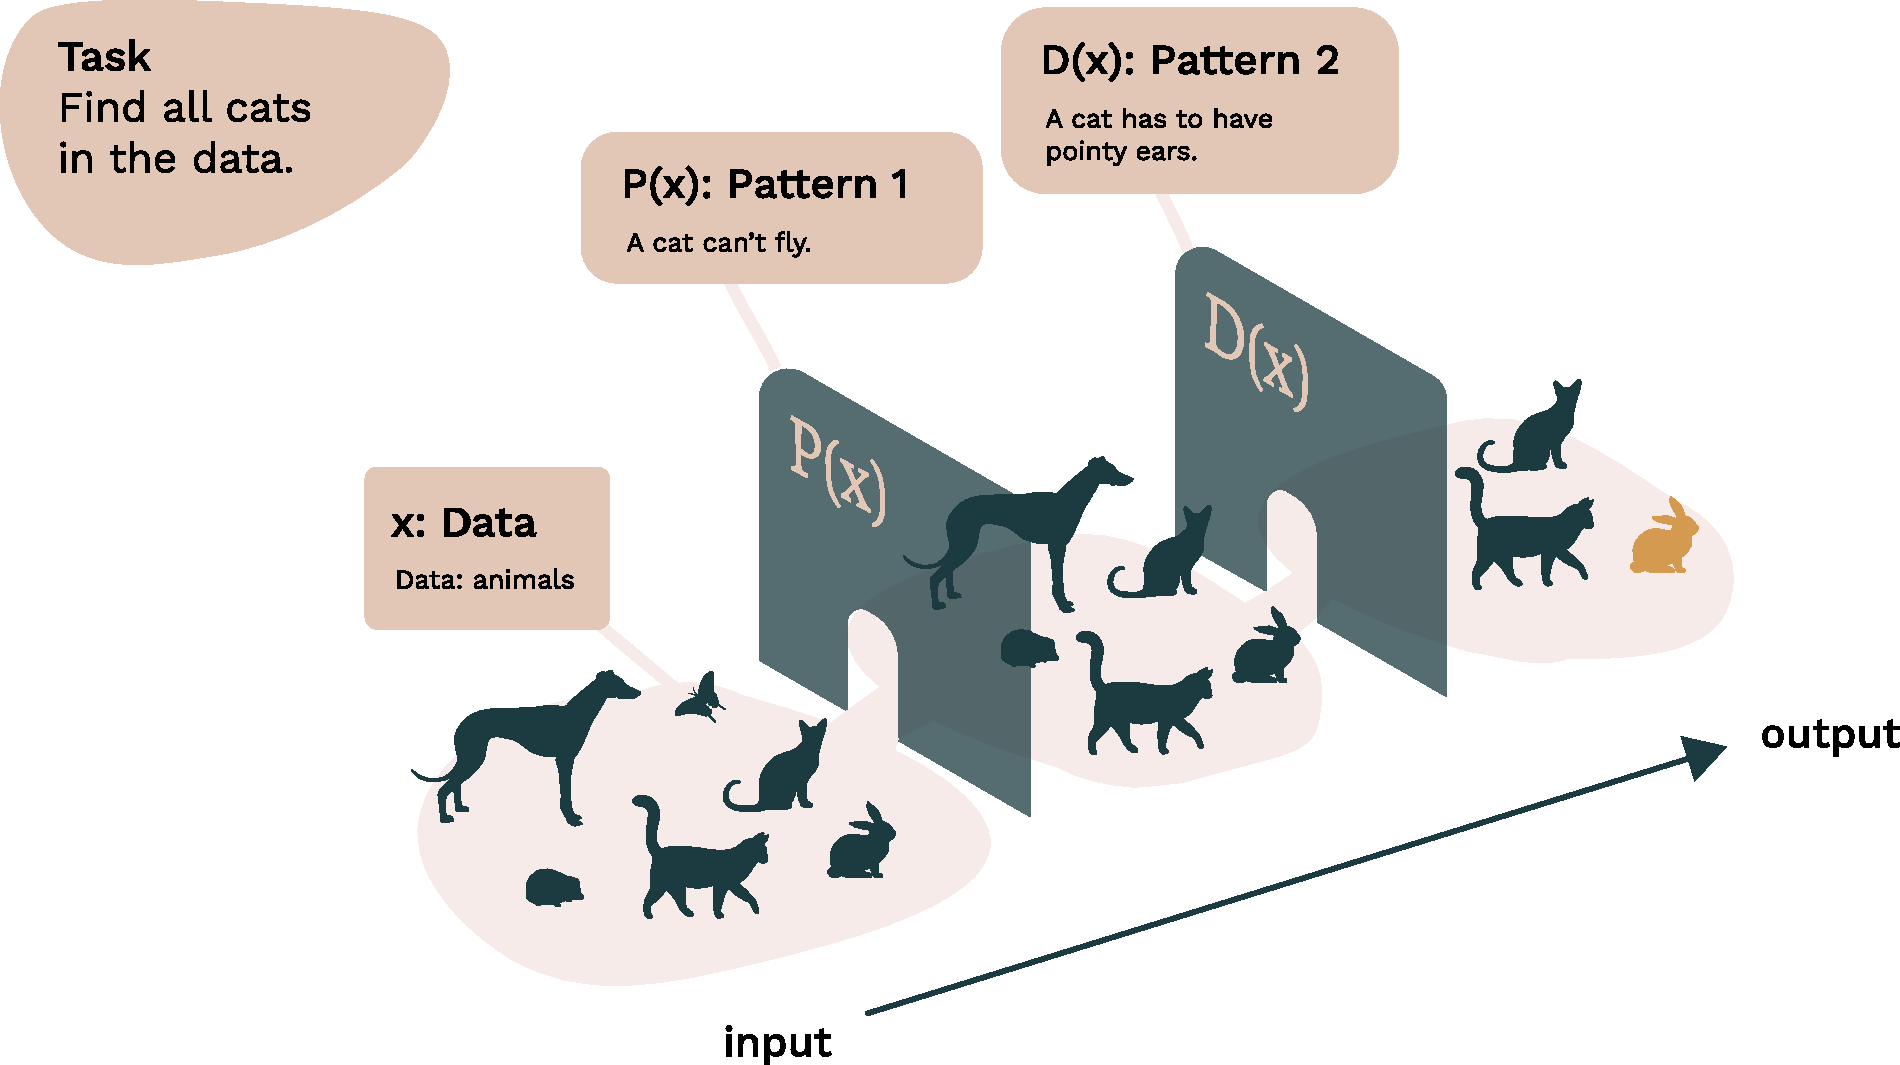
\includegraphics[keepaspectratio,alt={Autópsia de um modelo}]{img/autopsy.pdf}}
\caption{Autópsia de um modelo}
\end{figure}

Esta ilustração retrata um modelo de IA muito simplificado, encarregado
de reconhecer todos os gatos em dados compostos por animais de todo
tipo. O modelo inferiu dois padrões que compõem um gato. Para o modelo,
são apenas números; para nós, parecem padrões descritíveis. Contudo, os
padrões e características inferidos podem parecer bastante complicados
para nós. Para mais informações, veja
\url{https://distill.pub/2017/feature-visualization/}.

Além disso, a transparência cumpre muitas outras funções nos debates
contemporâneos sobre modelos de aprendizado de máquina. Pode ser
relevante para o desenvolvimento de legislação ou para assegurar a
confiança pública na IA. Para lidar com essas questões, a noção de
transparência em IA costuma receber uma definição mais ampla, em termos
de ``compreensibilidade''.

\subsubsection{A transparência como
compreensibilidade}\label{a-transparuxeancia-como-compreensibilidade}

A compreensibilidade de um algoritmo exige que se explique como uma
decisão foi tomada por um modelo de IA de maneira suficientemente
compreensível para os afetados por ele. É preciso ter uma noção concreta
de como ou por que determinada decisão foi alcançada a partir das
entradas.

No entanto, é notoriamente difícil traduzir conceitos derivados
algoritmicamente em conceitos compreensíveis por humanos. Em alguns
países, legisladores discutiram se as autoridades públicas deveriam
publicar os algoritmos que usam em decisões automatizadas na forma de
código de programação. Contudo, a maioria das pessoas não sabe
interpretar código. É difícil, portanto, ver como a transparência
aumentaria com a publicação de códigos.

\begin{Shaded}
\begin{Highlighting}[]
\NormalTok{* Toma o número da semente a partir do relógio da máquina;}
\NormalTok{data \_NULL\_;}
\NormalTok{ seedNumber= int(\%sysfunc(TIME())) ;}
\NormalTok{ call symput(\textquotesingle{}seedNumber\textquotesingle{},seedNumber);}
\NormalTok{run;}
\NormalTok{\%put \&seedNumber;}

\NormalTok{* Ordena o universo;}
\NormalTok{proc sort data=universe;}
\NormalTok{ by henro;}
\NormalTok{run;}
\NormalTok{* Cria uma amostra, n=2000;}
\NormalTok{proc surveyselect data=universe method=srs}
\NormalTok{     n=2000 seed=\&seedNumber}
\NormalTok{     out=sample;}
\NormalTok{run;}
\NormalTok{* Ordena a amostra;}
\NormalTok{proc sort data=sample;}
\NormalTok{ by henro;}
\NormalTok{run;}

\NormalTok{ * Une a amostra ao universo e cria a variável TYPE;}
\NormalTok{data all;}
\NormalTok{ merge universe(in=a)}
\NormalTok{       sample(in=b);}
\NormalTok{ by henro;}
\NormalTok{ length TYPE $ 1.;}
\NormalTok{ if a then TYPE=\textquotesingle{}V\textquotesingle{}; * grupo de referência;}
\NormalTok{ if b then TYPE=\textquotesingle{}K\textquotesingle{}; * grupo experimental;}

\NormalTok{ * atribui valores à variável REAOH;}
\NormalTok{REAOH=\textquotesingle{}PUOTOS\textquotesingle{};}
\NormalTok{run;}

\NormalTok{* Confirma que todas as 2000 pessoas têm TYPE com valor \textquotesingle{}K\textquotesingle{};}
\NormalTok{proc freq;}
\NormalTok{ tables type;}
\NormalTok{run;}
\end{Highlighting}
\end{Shaded}

Seria mais útil publicar os algoritmos exatos? Na maioria dos casos,
publicar os algoritmos exatos também não traz muita transparência,
especialmente se não se tem acesso aos dados usados no modelo.

\begin{figure}
\centering
\pandocbounded{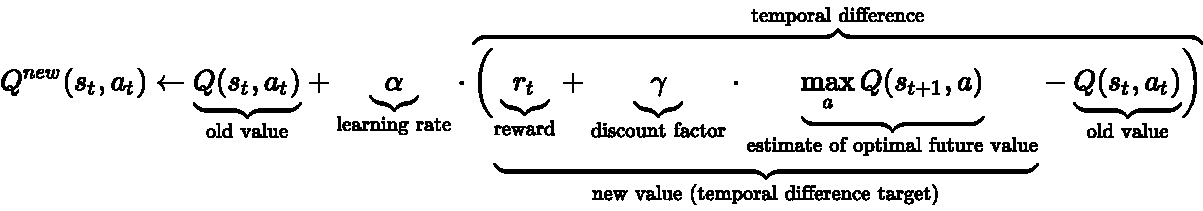
\includegraphics[keepaspectratio,alt={Aprendizado por reforço (Q-learning)}]{img/q-learning.pdf}}
\caption{Aprendizado por reforço (Q-learning)}
\end{figure}

Atualmente, cientistas cognitivos e da computação desenvolvem descrições
interpretáveis por humanos sobre como as aplicações se comportam e por
quê. As abordagens incluem, por exemplo, o desenvolvimento de
ferramentas de visualização de dados, interfaces interativas,
explicações verbais ou descrições em metanível das características dos
modelos. Essas ferramentas podem ser extremamente úteis para tornar as
aplicações de IA mais acessíveis. Ainda assim, há muito trabalho a ser
feito.

\begin{figure}
\centering
\pandocbounded{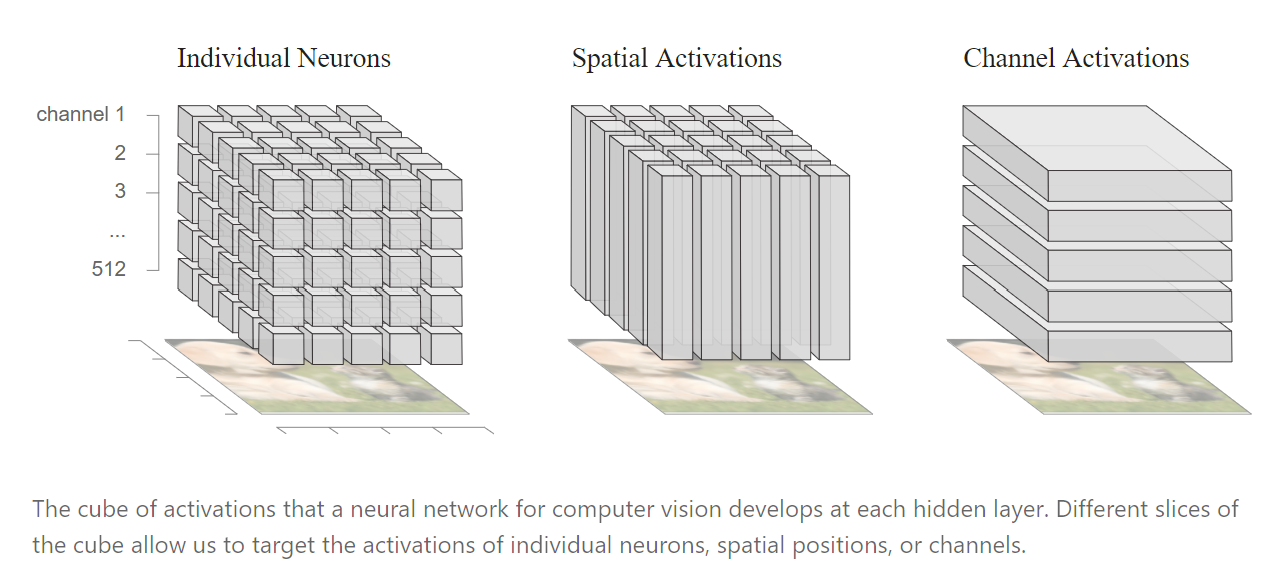
\includegraphics[keepaspectratio,alt={Exemplo do Distill}]{img/distill-example.png}}
\caption{Exemplo do Distill}
\end{figure}

\emph{Diagrama CC BY 4.0 Olah et al., ``The Building Blocks of
Interpretability'', Distill, 2018.}

O fato de a compreensibilidade se apoiar em componentes dependentes do
sujeito e da cultura complica ainda mais o quadro. Por exemplo, a lógica
de como visualizações são interpretadas --- ou de como inferências são
feitas a partir delas --- varia entre culturas. Assim, desenvolvedores
devem prestar atenção à compreensão suficiente da linguagem visual que
empregam.

Além disso, muito depende do grau de letramento em dados ou algoritmos,
por exemplo do conhecimento das tecnologias contemporâneas. Em algumas
culturas, o vocabulário da tecnologia atual é mais familiar; em muitas
outras, pode ser completamente novo. Para aumentar a compreensibilidade,
há uma necessidade clara de esforços educacionais significativos na
melhoria do letramento algorítmico --- por exemplo, em ``pensamento
computacional''
(\href{https://ieeexplore.ieee.org/document/7757410}{Heintz et al.,
2016}). Esse letramento do usuário terá efeito direto sobre a
transparência, no sentido da compreensão básica que os usuários comuns
têm dos sistemas de IA. Pode ser, na prática, o modo mais eficiente e
concreto de tornar as caixas menos pretas para muita gente.

\begin{tecnica}[Como tornar modelos mais transparentes?]

O problema da caixa-preta da inteligência artificial não é novo. Prover
transparência a modelos de aprendizado de máquina é uma área ativa de
pesquisa. Grosso modo, há cinco abordagens principais:

\begin{itemize}
\item
  \textbf{Usar modelos mais simples.} Isso, porém, com frequência
  sacrifica acurácia em troca de explicabilidade.
\item
  \textbf{Combinar modelos simples e sofisticados.} Enquanto o modelo
  sofisticado permite ao sistema realizar cálculos mais complexos, o
  modelo simples pode ser usado para prover transparência.
\item
  \textbf{Modificar as entradas para rastrear dependências relevantes
  entre entradas e saídas.} Se a manipulação das entradas altera os
  resultados gerais do modelo, essas entradas podem ter papel na
  classificação.
\item
  \textbf{Projetar os modelos para o usuário.} Isso requer usar métodos
  e ferramentas cognitiva e psicologicamente eficientes para visualizar
  os estados do modelo ou dirigir a atenção. Por exemplo, em visão
  computacional, estados em camadas intermediárias dos modelos podem ser
  visualizados como características (cabeças, braços, pernas),
  oferecendo uma descrição compreensível para a classificação de
  imagens. Pesquisadores também desenvolveram métodos para dirigir a
  ``atenção'' às partes da entrada que mais importam. Elas podem ser
  visualizadas para destacar as partes de uma imagem ou de um texto (os
  chamados ``pesos'') que mais contribuem para determinada recomendação.
\item
  \textbf{Acompanhar a pesquisa mais recente.} Há muita pesquisa em
  curso sobre diversos aspectos da IA explicável --- incluindo as
  dimensões sociocognitivas --- e novas técnicas vêm sendo
  desenvolvidas.
\end{itemize}

\end{tecnica}

\begin{reflexao}[Exercícios desta seção]

O material original traz aqui um questionário interativo. As perguntas
não constam do repositório de origem --- ficam no banco de dados da
plataforma. O exercício correspondente deve ser redigido em
\texttt{exercicios/capitulo04-exercicios.md}.

\end{reflexao}

\subsubsection{Estudo de caso: três visualizações do mesmo
algoritmo}\label{estudo-de-caso-truxeas-visualizauxe7uxf5es-do-mesmo-algoritmo}

\begin{caso}[Qual delas é compreensível?]

Há necessidade de traduzir conceitos algorítmicos para a linguagem
cotidiana. A maioria das pessoas sem formação em computação não conhece
o vocabulário básico da IA, o que afeta diretamente sua capacidade de
compreender os desenvolvimentos recentes.

\textbf{1.}

\begin{figure}
\centering
\pandocbounded{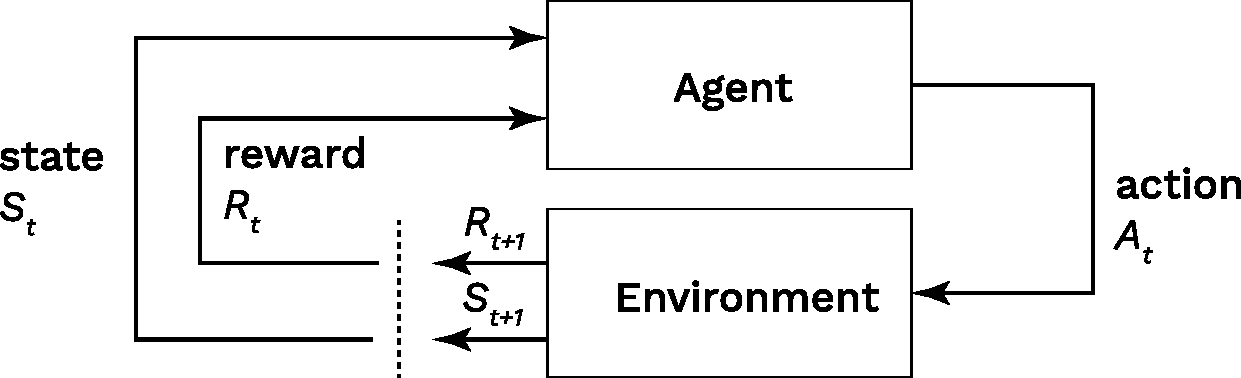
\includegraphics[keepaspectratio,alt={Algoritmo de aprendizado por reforço --- versão técnica}]{img/rl1.pdf}}
\caption{Algoritmo de aprendizado por reforço --- versão técnica}
\end{figure}

\textbf{2.}

\begin{figure}
\centering
\pandocbounded{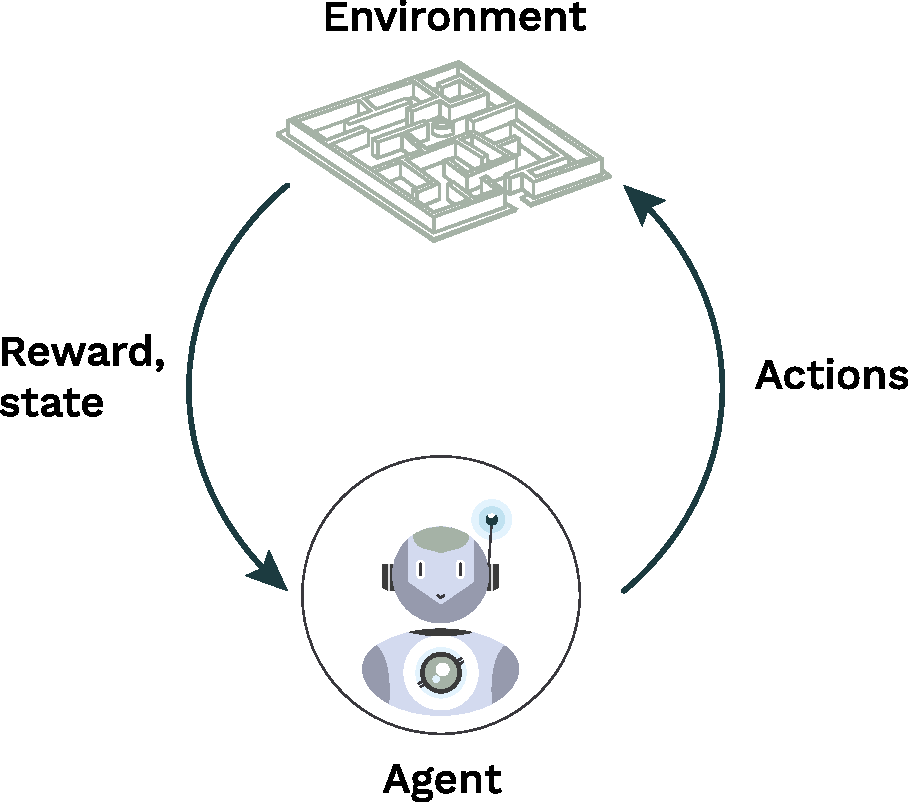
\includegraphics[keepaspectratio,alt={Algoritmo de aprendizado por reforço --- versão com robô}]{img/rl2.pdf}}
\caption{Algoritmo de aprendizado por reforço --- versão com robô}
\end{figure}

\textbf{3.}

\begin{figure}
\centering
\pandocbounded{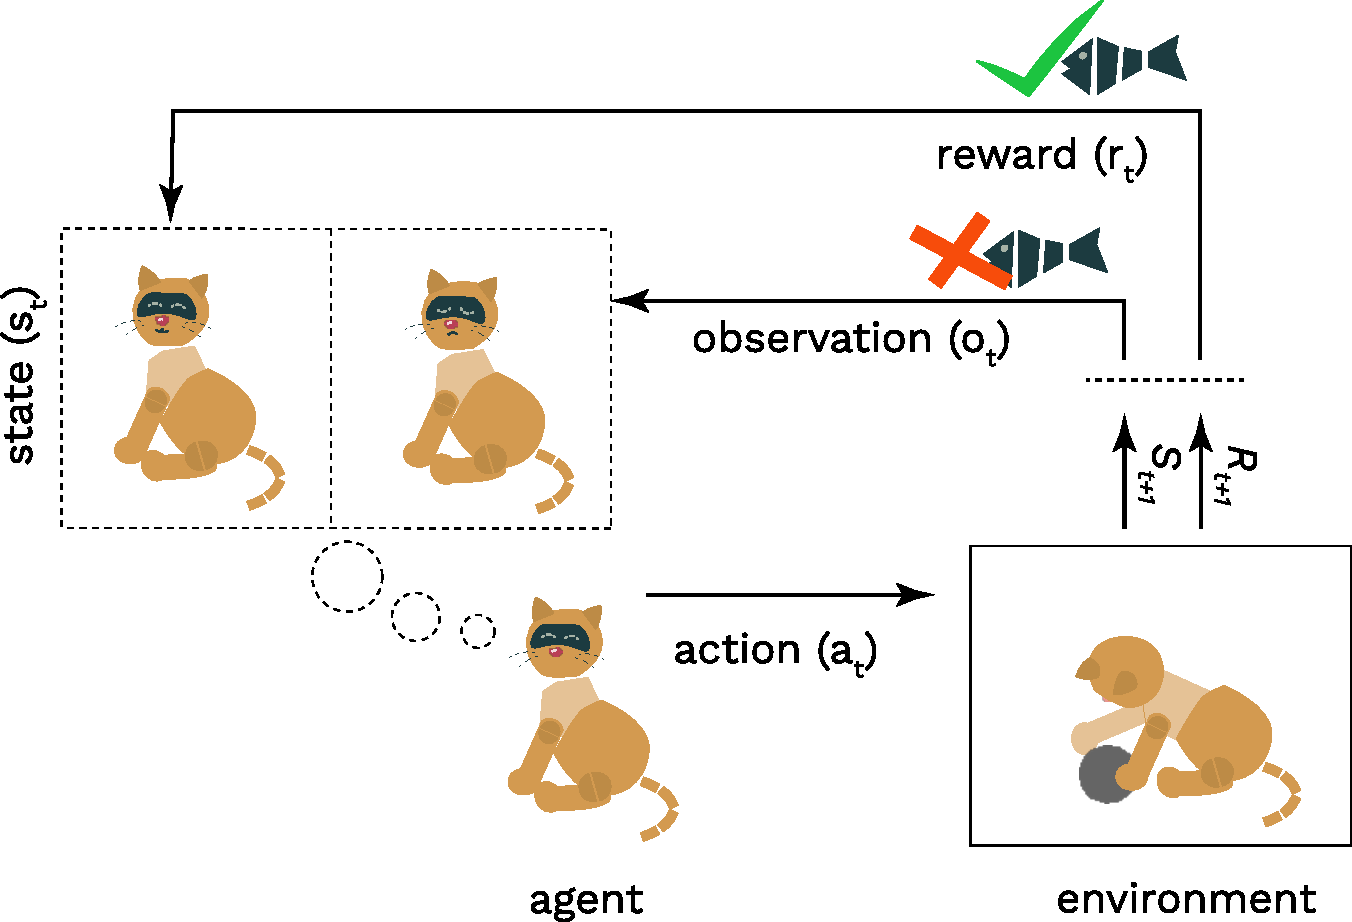
\includegraphics[keepaspectratio,alt={Algoritmo de aprendizado por reforço --- versão com gato}]{img/rl3.pdf}}
\caption{Algoritmo de aprendizado por reforço --- versão com gato}
\end{figure}

Compare estas três visualizações de algoritmos de aprendizado por
reforço. Qual delas é a mais compreensível? Por quê?

\end{caso}

\subsection{III. Transparência e os riscos da
abertura}\label{iii.-transparuxeancia-e-os-riscos-da-abertura}

A transparência frequentemente denota um ``ideal'' ético, social e
jurídico moderno (Koivisto, 2016), uma exigência normativa para o uso
aceitável da tecnologia em nossas sociedades. É um reflexo do ideal de
``abertura'', formulado em termos de ``governo aberto'', ``dados
abertos'', ``código aberto/acesso aberto'', bem como ``ciência aberta''
(Larsson, 2020). Nesse sentido, considerações sobre transparência são
necessárias para favorecer a distribuição equitativa dos avanços
científicos, de modo que os benefícios do desenvolvimento da IA possam
ser acessíveis a todas as pessoas.

\begin{nota}[O paradoxo da abertura]

Paradoxalmente, o ideal de abertura também pode levar a consequências
danosas. Por exemplo, a transparência das plataformas de redes sociais
levou a diversos casos de uso indevido e a desafios democráticos. A
transparência pode criar riscos de segurança. Transparência demais pode
levar ao vazamento de dados sensíveis à privacidade para as mãos
erradas. Ou ainda: quanto mais se revela sobre os algoritmos e os dados,
mais dano um ator malicioso pode causar. Algoritmos podem ser invadidos,
e a informação pode tornar a IA mais vulnerável a ataques intencionais.
Algoritmos inteiros também podem ser roubados apenas a partir de suas
explicações.

\end{nota}

Em resumo, embora haja necessidade de desenvolver práticas mais
transparentes para a IA, também é preciso desenvolver práticas que
ajudem a evitar abusos. Ainda que a transparência possa ajudar a mitigar
questões éticas --- como equidade ou responsabilização
(\emph{accountability}) ---, ela também cria riscos eticamente
importantes. Abertura demais no contexto errado pode frustrar o
desenvolvimento positivo de processos habilitados por IA. Em conjunto,
fica claro que o ideal de transparência total dos algoritmos deve ser
considerado com cuidado, e será preciso encontrar um equilíbrio entre as
exigências de segurança e as de transparência.

\begin{reflexao}[Exercícios desta seção]

O material original traz aqui um questionário interativo. As perguntas
não constam do repositório de origem. O exercício correspondente deve
ser redigido em \texttt{exercicios/capitulo04-exercicios.md}.

\end{reflexao}

\subsection{Referências}\label{referuxeancias}

Heintz, F., Mannila, L., \& Färnqvist, T. (2016). A review of models for
introducing computational thinking, computer science and computing in
K-12 education. \emph{IEEE Frontiers in Education Conference}.
\url{https://ieeexplore.ieee.org/document/7757410}

Koivisto, I. (2016). The anatomy of transparency: The concept and its
multifarious implications.

Larsson, S. (2020). On the governance of artificial intelligence through
ethics guidelines.

Olah, C., et al.~(2018). The Building Blocks of Interpretability.
\emph{Distill}. \url{https://distill.pub/2018/building-blocks/}

Rusanen, A.-M., \& Ylikoski, P. (2017).

Wachter, S., Mittelstadt, B., \& Russell, C. (2018). Counterfactual
Explanations Without Opening the Black Box: Automated Decisions and the
GDPR. \url{https://arxiv.org/pdf/1811.01439.pdf}

\begin{center}\rule{0.5\linewidth}{0.5pt}\end{center}

\begin{licenca}

\textbf{Material original:} \emph{Ethics of AI}, um curso online
gratuito da Universidade de Helsinque. Professores responsáveis:
Anna-Mari Rusanen e Jukka K. Nurminen. Demais contribuintes principais:
Santeri Räisänen, Sasu Tarkoma e Saara Halmetoja. Disponível em
\url{https://ethics-of-ai.mooc.fi/}.

\textbf{Esta versão:} tradução e adaptação para o português brasileiro
realizada por José Lucas Lira Bizil, Fernando Mazzeto Lisboa Lima e
Matheus da Silva Fernandes, no âmbito do Programa CiberExt 26-29
(FEELT38103), Universidade Federal de Uberlândia, 2026. Esta é uma obra
derivada; os autores originais não a revisaram nem a endossam.

\textbf{Licença:} Creative Commons
Atribuição-NãoComercial-CompartilhaIgual 4.0 Internacional (CC BY-NC-SA
4.0) ---
\url{https://creativecommons.org/licenses/by-nc-sa/4.0/deed.pt-br}.

\end{licenca}

\end{document}
